\documentclass[12pt, mathserif,handout]{beamer}
\usepackage{etex}


\usepackage{agda}

\usepackage{mypack}

\usepackage{ucs}
\usepackage[utf8x]{inputenc}

\usepackage{relsize}
\usepackage{autofe}
\usepackage{textgreek}

\setbeamertemplate{navigation symbols}{}


\usetheme{Berlin}
\setbeamercovered{highly dynamic} 
\usepackage{xspace}
\usepackage{ifthen}
\usepackage{amsmath}
\usepackage{amssymb}
\usepackage{stmaryrd}
\usepackage{proof}

\usepackage[english]{babel}
\usepackage{graphicx}
\usepackage{multimedia}
\usepackage{animate}
\usepackage[all]{xy}
\usepackage{booktabs}
\usepackage[nobibnewpage,notocbib]{apacite}
\usepackage[absolute,overlay,quiet]{textpos}

\definecolor{blueish}{rgb}{0.2, 0.2, 0.7}

\usepackage[T1]{fontenc}
\usepackage{cmbright}
\usepackage{fancybox}

\usepackage[inference]{semantic}

% Background Color

\definecolor{rice}{RGB}{245,245,220}
\setbeamercolor{background canvas}{bg=rice}

\setbeamercolor{yellow}{fg=black,bg=yellow}
\setbeamercolor{lightyellow}{fg=black,bg=yellow!40}
\setbeamercolor{orange}{fg=black,bg=orange}
\setbeamercolor{lightorange}{fg=black,bg=orange!40}
\setbeamercolor{green}{fg=black,bg=green}
\setbeamercolor{lightgreen}{fg=black,bg=green!40}
\setbeamercolor{blue}{fg=black,bg=blue}
\setbeamercolor{lightblue}{fg=black,bg=blue!40}
\setbeamercolor{red}{fg=black,bg=red}
\setbeamercolor{lightred}{fg=black,bg=red!40}
\setbeamercolor{lightpink}{fg=black,bg=pink!40}


%\setbeamercolor{frametitle}{fg=white,bg=orange}
%\setbeamercolor{title}{fg=white,bg=orange}

\setbeamercovered{invisible}

%\begin{colorblock}{orange}{lightyellow}{\center{Heterogeneous equality for Tm}}


\newenvironment{colorblock}[2]
{\setbeamercolor{item}{fg=#1,bg=#1}\begin{beamerboxesrounded}[upper=#1,lower=#2,shadow=true]}
{\end{beamerboxesrounded}}



% shorthands


\author{Thorsten Altenkirch \& Nuo Li \& Ond\v{r}ej Ryp\'a\v{c}ek}

\author[Thorsten Altenkirch \& Nuo Li \& Ond\v{r}ej
Ryp\'a\v{c}ek]{Thorsten Altenkirch \inst{1} \and Nuo Li \inst{1} \and
  Ond\v{r}ej Ryp\'a\v{c}ek \inst{2}}
\institute[shortinst]{\inst{1} 
School of Computer Science \\  University of Nottingham, UK \and %
                      \inst{2} University of Oxford, UK}






\date[17/07/14]{17/07/14}
\title{Some constructions on $\omega$-groupoids}
\subtitle[LFMTP 2014]{}


\addtobeamertemplate{sidebar right}{}{\vspace{-2cm}}
\addtobeamertemplate{footline}{}{\vspace{-1cm}\hskip2pt(\insertframenumber/\inserttotalframenumber) \insertshortsubtitle{} -- \insertshortdate\vskip2.2pt}
\setbeamercolor{footline}{fg=purple}


\begin{document}

% 1
\frame{\titlepage}


% 2

\begin{frame}{Outline}
\begin{itemize}
\item What are \wog?
\item Basic syntax
\item Heterogeneous Equality for syntactic terms
\item Rules and lemmas
\item Some advanced construction
\item Suspensions and groupoid laws
\item Semantics
\end{itemize}
\end{frame}




\begin{frame}[allowframebreaks,t]{Introduction to \wog}

\begin{itemize}
\item \hott is a new branch between mathematics and computer science
\begin{itemize}
\item{Univalent axiom: equality of types is weakly equivalent to weak equivalence}
\end{itemize}
\pause

\item In \hott, types bear the structure of weak $\omega$-groupoids
\begin{itemize}
\item Generalisation of setoids, 1-groupoids, n-groupoidsd etc.
\item A higher dimensional category ($\omega$-category) : every
  morphism is an (weak) equivalence
\item Equivalence:
\item Weak equivalence: invertible morphism up to all higher
  equivalence, generalisation of isomorphism
\item Weak: equality in coherence laws are up to equivalence (not
    strictly equal) e.g. $(f \circ g) \circ h \to f \circ (g \circ h)$
\end{itemize}

\item Related work:
\begin{itemize}
\item{Grothendieck's definition in 1983}
\item{Maltsiniotis and Ara simplified the original definition}
\pause
\item In Type Theory:
\begin{itemize}
\item Hofmann and Streicher's groupoid model of type
  theory
\item Warren's strict $\omega$-groupoid model
\item Altenkirch and Rypacek's syntactic approach
\item Brunerie's proposal to encode Grothendieck's definition using
  a type theory called \tig
\end{itemize}

\end{itemize}


\end{frame}





\begin{frame}[allowframebreaks,t]{Coherences}

\begin{itemize}

\item They are morphisms in \wog
\item Setoid: 
\begin{equation*}
\begin{array}[b]{l} 
\text{id} : x = x \\
\_^{-1} : x= y \to y  = x \\
\_ \circ\_ : y = z \to x = y \to x = z
 \end{array}
\end{equation*}

\item Groupoid: 

\begin{equation*}
\begin{array}[b]{l}
\lambda : id \circ p = p \\
\rho : p \circ id = p \\
\alpha : p \circ (q \circ r) = (p \circ q) \circ r \\
\kappa : p^{-1}\circ p = id \\
\kappa' : p \circ p^{-1} = id
 \end{array}
\end{equation*}
\item In \wog, We have an infiite tower of coherences 
\end{itemize}

\xymatrix{ 
a
\ar@/_4pc/[ddd]^p="p" 
\\
\\
\\
b 
\ar@/_4pc/[uuu]^{p^{-1}}="p^{-1}"" 
\only<2->{\ar@2{->} @/^2pc/ "p";"p^{-1}" _{H}="H"}
\only<3->{\ar@2{<-} @/_2pc/ "p";"p^{-1}" ^{H ^{-1}}="H^{-1}"}
\only<4->{\ar@3{->} @/^1pc/ "H";"H^{-1}"_{...}="A"}
\only<5->{\ar@3{<-}@/_1pc/  "H";"H^{-1}"^{...}="A"}
}


How can we decribe all these coherences laws in \wog?



%\begin{columns}[c]

% \begin{column}{2cm}


% 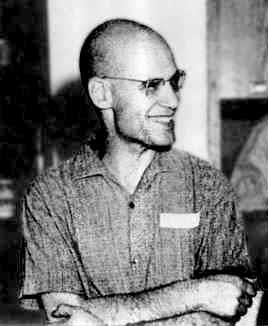
\includegraphics[scale=0.2]{Alexander_Grothendieck.jpg}

% \end{column}



%\begin{column}{3cm}

%\end{column}

%\end{columns}

% \item{Grothendieck introduced the notion of \og{} in 1983 in a
%     manuscript called \emph{Pursuing Stacks}} 
% \pause

\end{frame}



% 3


% 4



% \begin{frame}{Agda}
% \begin{itemize}
% \item A functional programming language
% \item An implementation of intensional \mltt
% \item Dependent types
% \item $\Pi$-types : $(x : A) \to B$
% \item Implict argument : $\{x : A\} \to B$
% \item Unicode support \& mixfix definitions e.g. $\_⇒\_$
% \item Inductive inductive definitions
% \item Coinductive definitions
% \end{itemize}
% \end{frame}


\begin{frame}[allowframebreaks,t]{Basic syntax}

\begin{itemize}
\item The definition is interdependent

\item A feature of Agda for defining types inductive inductively

\item We declare the type signature first:

\begin{code}\>\<
\\
\>\AgdaKeyword{data} \AgdaDatatype{Con} \<[19]%
\>[19]\AgdaSymbol{:} \AgdaPrimitiveType{Set}\<%
\\
\>\AgdaKeyword{data} \AgdaDatatype{Ty} \AgdaSymbol{(}\AgdaBound{Γ} \AgdaSymbol{:} \AgdaDatatype{Con}\AgdaSymbol{)} \<[19]%
\>[19]\AgdaSymbol{:} \AgdaPrimitiveType{Set}\<%
\\
\>\AgdaKeyword{data} \AgdaDatatype{Tm} \<[19]%
\>[19]\AgdaSymbol{:} \AgdaSymbol{\{}\AgdaBound{Γ} \AgdaSymbol{:} \AgdaDatatype{Con}\AgdaSymbol{\}(}\AgdaBound{A} \AgdaSymbol{:} \AgdaDatatype{Ty} \AgdaBound{Γ}\AgdaSymbol{)} \AgdaSymbol{→} \AgdaPrimitiveType{Set}\<%
\\
\>\AgdaKeyword{data} \AgdaDatatype{Var} \<[19]%
\>[19]\AgdaSymbol{:} \AgdaSymbol{\{}\AgdaBound{Γ} \AgdaSymbol{:} \AgdaDatatype{Con}\AgdaSymbol{\}(}\AgdaBound{A} \AgdaSymbol{:} \AgdaDatatype{Ty} \AgdaBound{Γ}\AgdaSymbol{)} \AgdaSymbol{→} \AgdaPrimitiveType{Set}\<%
\\
\>\AgdaKeyword{data} \AgdaDatatype{\_⇒\_} \<[19]%
\>[19]\AgdaSymbol{:} \AgdaDatatype{Con} \AgdaSymbol{→} \AgdaDatatype{Con} \AgdaSymbol{→} \AgdaPrimitiveType{Set}\<%
\\
\>\AgdaKeyword{data} \AgdaDatatype{isContr} \<[19]%
\>[19]\AgdaSymbol{:} \AgdaDatatype{Con} \AgdaSymbol{→} \AgdaPrimitiveType{Set}\<%
\\
\>\<\end{code}
% 6

\item and then definitions:
\end{itemize}

\small{
\begin{code}\>\<%
\\
\>\AgdaKeyword{data} \AgdaDatatype{Con} \AgdaKeyword{where}\<%
\\
\>[0]\AgdaIndent{2}{}\<[2]%
\>[2]\AgdaInductiveConstructor{ε} \<[6]%
\>[6]\AgdaSymbol{:} \AgdaDatatype{Con}\<%
\\
\>[0]\AgdaIndent{2}{}\<[2]%
\>[2]\AgdaInductiveConstructor{\_,\_} \AgdaSymbol{:} \AgdaSymbol{(}\AgdaBound{Γ} \AgdaSymbol{:} \AgdaDatatype{Con}\AgdaSymbol{)(}\AgdaBound{A} \AgdaSymbol{:} \AgdaDatatype{Ty} \AgdaBound{Γ}\AgdaSymbol{)} \AgdaSymbol{→} \AgdaDatatype{Con}\<%
\\
%
\\
\>\AgdaKeyword{data} \AgdaDatatype{Ty} \AgdaBound{Γ} \AgdaKeyword{where}\<%
\\
\>[0]\AgdaIndent{2}{}\<[2]%
\>[2]\AgdaInductiveConstructor{*} \<[6]%
\>[6]\AgdaSymbol{:} \AgdaDatatype{Ty} \AgdaBound{Γ}\<%
\\
\>[0]\AgdaIndent{2}{}\<[2]%
\>[2]\AgdaInductiveConstructor{\_=h\_} \AgdaSymbol{:} \AgdaSymbol{\{}\AgdaBound{A} \AgdaSymbol{:} \AgdaDatatype{Ty} \AgdaBound{Γ}\AgdaSymbol{\}(}\AgdaBound{a} \AgdaBound{b} \AgdaSymbol{:} \AgdaDatatype{Tm} \AgdaBound{A}\AgdaSymbol{)} \AgdaSymbol{→} \AgdaDatatype{Ty} \AgdaBound{Γ}\<%
\\
%
\\
\>\AgdaKeyword{data} \AgdaDatatype{Var} \AgdaKeyword{where}\<%
\\
\>[1]\AgdaIndent{2}{}\<[2]%
\>[2]\AgdaInductiveConstructor{v0} \AgdaSymbol{:} \AgdaSymbol{\{}\AgdaBound{Γ} \AgdaSymbol{:} \AgdaDatatype{Con}\AgdaSymbol{\}\{}\AgdaBound{A} \AgdaSymbol{:} \AgdaDatatype{Ty} \AgdaBound{Γ}\AgdaSymbol{\}} \<[40]%
\>[40]\AgdaSymbol{→} \AgdaDatatype{Var} \AgdaSymbol{(}\AgdaBound{A} \AgdaFunction{+T} \AgdaBound{A}\AgdaSymbol{)}\<%
\\
\>[0]\AgdaIndent{2}{}\<[2]%
\>[2]\AgdaInductiveConstructor{vS} \AgdaSymbol{:} \AgdaSymbol{\{}\AgdaBound{Γ} \AgdaSymbol{:} \AgdaDatatype{Con}\AgdaSymbol{\}\{}\AgdaBound{A} \AgdaBound{B} \AgdaSymbol{:} \AgdaDatatype{Ty} \AgdaBound{Γ}\AgdaSymbol{\}(}\AgdaBound{x} \AgdaSymbol{:} \AgdaDatatype{Var} \AgdaBound{A}\AgdaSymbol{)} \AgdaSymbol{→} \AgdaDatatype{Var} \AgdaSymbol{(}\AgdaBound{A} \AgdaFunction{+T} \AgdaBound{B}\AgdaSymbol{)}\<%
\\
%
\\
\>\AgdaKeyword{data} \AgdaDatatype{Tm} \AgdaKeyword{where}\<%
\\
\>[0]\AgdaIndent{2}{}\<[2]%
\>[2]\AgdaInductiveConstructor{var} \AgdaSymbol{:} \AgdaSymbol{\{}\AgdaBound{Γ} \AgdaSymbol{:} \AgdaDatatype{Con}\AgdaSymbol{\}\{}\AgdaBound{A} \AgdaSymbol{:} \AgdaDatatype{Ty} \AgdaBound{Γ}\AgdaSymbol{\}} \AgdaSymbol{→} \AgdaDatatype{Var} \AgdaBound{A} \AgdaSymbol{→} \AgdaDatatype{Tm} \AgdaBound{A}\<%
\\
\>[0]\AgdaIndent{2}{}\<[2]%
\>[2]\AgdaInductiveConstructor{coh} \<[6]%
\>[6]\AgdaSymbol{:} \AgdaSymbol{\{}\AgdaBound{Γ} \AgdaBound{Δ} \AgdaSymbol{:} \AgdaDatatype{Con}\AgdaSymbol{\}} \AgdaSymbol{→} \AgdaDatatype{isContr} \AgdaBound{Δ} \AgdaSymbol{→} \AgdaSymbol{(}\AgdaBound{δ} \AgdaSymbol{:} \AgdaBound{Γ} \AgdaDatatype{⇒} \AgdaBound{Δ}\AgdaSymbol{)} \AgdaSymbol{→} \AgdaSymbol{(}\AgdaBound{A} \AgdaSymbol{:} \AgdaDatatype{Ty} \AgdaBound{Δ}\AgdaSymbol{)} \<[59]%
\>[59]\<%
\\
\>[2]\AgdaIndent{6}{}\<[6]%
\>[6]\AgdaSymbol{→} \AgdaDatatype{Tm} \AgdaSymbol{(}\AgdaBound{A} \AgdaFunction{[} \AgdaBound{δ} \AgdaFunction{]T}\AgdaSymbol{)}\<%
\\
%
\\
\>\AgdaKeyword{data} \AgdaDatatype{isContr} \AgdaKeyword{where}\<%
\\
\>[0]\AgdaIndent{2}{}\<[2]%
\>[2]\AgdaInductiveConstructor{c*} \<[6]%
\>[6]\AgdaSymbol{:} \AgdaDatatype{isContr} \AgdaSymbol{(}\AgdaInductiveConstructor{ε} \AgdaInductiveConstructor{,} \AgdaInductiveConstructor{*}\AgdaSymbol{)}\<%
\\
\>[0]\AgdaIndent{2}{}\<[2]%
\>[2]\AgdaInductiveConstructor{ext} \AgdaSymbol{:} \AgdaSymbol{\{}\AgdaBound{Γ} \AgdaSymbol{:} \AgdaDatatype{Con}\AgdaSymbol{\}} \<[18]%
\>[18]\<%
\\
\>[2]\AgdaIndent{6}{}\<[6]%
\>[6]\AgdaSymbol{→} \AgdaDatatype{isContr} \AgdaBound{Γ} \AgdaSymbol{→} \AgdaSymbol{\{}\AgdaBound{A} \AgdaSymbol{:} \AgdaDatatype{Ty} \AgdaBound{Γ}\AgdaSymbol{\}(}\AgdaBound{x} \AgdaSymbol{:} \AgdaDatatype{Var} \AgdaBound{A}\AgdaSymbol{)} \<[42]%
\>[42]\<%
\\
\>[6]\AgdaIndent{8}{}\<[8]%
\>[8]\AgdaSymbol{→} \AgdaDatatype{isContr} \AgdaSymbol{((}\AgdaBound{Γ} \AgdaInductiveConstructor{,} \AgdaBound{A}\AgdaSymbol{)} \AgdaInductiveConstructor{,} \AgdaSymbol{(}\AgdaInductiveConstructor{var} \AgdaSymbol{(}\AgdaInductiveConstructor{vS} \AgdaBound{x}\AgdaSymbol{)} \AgdaInductiveConstructor{=h} \AgdaInductiveConstructor{var} \AgdaInductiveConstructor{v0}\AgdaSymbol{))}\<%
\\%
\\
\>\AgdaKeyword{data} \AgdaDatatype{\_⇒\_} \AgdaKeyword{where}\<%
\\
\>[0]\AgdaIndent{2}{}\<[2]%
\>[2]\AgdaInductiveConstructor{•} \<[7]%
\>[7]\AgdaSymbol{:} \AgdaSymbol{\{}\AgdaBound{Γ} \AgdaSymbol{:} \AgdaDatatype{Con}\AgdaSymbol{\}} \AgdaSymbol{→} \AgdaBound{Γ} \AgdaDatatype{⇒} \AgdaInductiveConstructor{ε}\<%
\\
\>[0]\AgdaIndent{2}{}\<[2]%
\>[2]\AgdaInductiveConstructor{\_,\_} \AgdaSymbol{:} \AgdaSymbol{\{}\AgdaBound{Γ} \AgdaBound{Δ} \AgdaSymbol{:} \AgdaDatatype{Con}\AgdaSymbol{\}(}\AgdaBound{δ} \AgdaSymbol{:} \AgdaBound{Γ} \AgdaDatatype{⇒} \AgdaBound{Δ}\AgdaSymbol{)\{}\AgdaBound{A} \AgdaSymbol{:} \AgdaDatatype{Ty} \AgdaBound{Δ}\AgdaSymbol{\}(}\AgdaBound{a} \AgdaSymbol{:} \AgdaDatatype{Tm} \AgdaSymbol{(}\AgdaBound{A} \AgdaFunction{[} \AgdaBound{δ} \AgdaFunction{]T}\AgdaSymbol{))} \<[60]%
\>[60]\<%
\\
\>[2]\AgdaIndent{6}{}\<[6]%
\>[6]\AgdaSymbol{→} \AgdaBound{Γ} \AgdaDatatype{⇒} \AgdaSymbol{(}\AgdaBound{Δ} \AgdaInductiveConstructor{,} \AgdaBound{A}\AgdaSymbol{)}\<%
\\
\>\<\end{code}
}

\end{frame}




\begin{frame}

\frametitle{Heterogeneous equality for terms}
\begin{itemize}
\item{The first challenge:  technically too many "Subst"s when reasoning about terms. unable to proceed}
\item{We found that the equality of types is decidable : an h-set}
\item{The proof of the equality is unique. We could use heterogeneous equality for Tm which depends on Ty}
\end{itemize}

\begin{colorblock}{orange}{lightyellow}{\center{Heterogeneous equality for Tm}}

\begin{code}\>\<%
\\
\>\AgdaKeyword{data} \AgdaDatatype{\_≅\_} \AgdaSymbol{\{}\AgdaBound{Γ} \AgdaSymbol{:} \AgdaDatatype{Con}\AgdaSymbol{\}\{}\AgdaBound{A} \AgdaSymbol{:} \AgdaDatatype{Ty} \AgdaBound{Γ}\AgdaSymbol{\}} \<[29]%
\>[29]\<%
\\
\>[2]\AgdaIndent{9}{}\<[9]%
\>[9]\AgdaSymbol{:} \AgdaSymbol{\{}\AgdaBound{B} \AgdaSymbol{:} \AgdaDatatype{Ty} \AgdaBound{Γ}\AgdaSymbol{\}} \AgdaSymbol{→} \AgdaDatatype{Tm} \AgdaBound{A} \AgdaSymbol{→} \AgdaDatatype{Tm} \AgdaBound{B} \AgdaSymbol{→} \AgdaPrimitiveType{Set} \AgdaKeyword{where}\<%
\\
\>[0]\AgdaIndent{2}{}\<[2]%
\>[2]\AgdaInductiveConstructor{refl} \AgdaSymbol{:} \AgdaSymbol{(}\AgdaBound{b} \AgdaSymbol{:} \AgdaDatatype{Tm} \AgdaBound{A}\AgdaSymbol{)} \AgdaSymbol{→} \AgdaBound{b} \AgdaDatatype{≅} \AgdaBound{b}\<%
\\
\>\<\end{code}

\end{colorblock}

\end{frame}



\begin{frame}

\frametitle{Heterogeneous equality for terms 2}

\begin{colorblock}{orange}{lightyellow}{\center{"Coercion''(proof-irrelevant substitution)}}
\small{
\begin{code}\>\<%
\\
\>\AgdaFunction{\_⟦\_⟫} \AgdaSymbol{:} \AgdaSymbol{\{}\AgdaBound{Γ} \AgdaSymbol{:} \AgdaDatatype{Con}\AgdaSymbol{\}\{}\AgdaBound{A} \AgdaBound{B} \AgdaSymbol{:} \AgdaDatatype{Ty} \AgdaBound{Γ}\AgdaSymbol{\}(}\AgdaBound{a} \AgdaSymbol{:} \AgdaDatatype{Tm} \AgdaBound{B}\AgdaSymbol{)} \AgdaSymbol{→} \AgdaBound{A} \AgdaDatatype{≡} \AgdaBound{B} \AgdaSymbol{→} \AgdaDatatype{Tm} \AgdaBound{A}\<%
\\
\>\AgdaBound{a} \AgdaFunction{⟦} \AgdaInductiveConstructor{refl} \AgdaFunction{⟫} \AgdaSymbol{=} \AgdaBound{a}\<%
\\
\>\<\end{code}
}

\end{colorblock}

\begin{colorblock}{orange}{lightyellow}{\center{"Coherence Operator"}}

\small{
\begin{code}\>\<
%
\\
\>\AgdaFunction{cohOp} \AgdaSymbol{:} \AgdaSymbol{\{}\AgdaBound{Γ} \AgdaSymbol{:} \AgdaDatatype{Con}\AgdaSymbol{\}\{}\AgdaBound{A} \AgdaBound{B} \AgdaSymbol{:} \AgdaDatatype{Ty} \AgdaBound{Γ}\AgdaSymbol{\}\{}\AgdaBound{a} \AgdaSymbol{:} \AgdaDatatype{Tm} \AgdaBound{B}\AgdaSymbol{\}(}\AgdaBound{p} \AgdaSymbol{:} \AgdaBound{A} \AgdaDatatype{≡} \AgdaBound{B}\AgdaSymbol{)} \<[51]%
\>[51]\<%
\\
\>[0]\AgdaIndent{6}{}\<[6]%
\>[6]\AgdaSymbol{→} \AgdaBound{a} \AgdaFunction{⟦} \AgdaBound{p} \AgdaFunction{⟫} \AgdaDatatype{≅} \AgdaBound{a}\<%
\\
\>\AgdaFunction{cohOp} \AgdaInductiveConstructor{refl} \AgdaSymbol{=} \AgdaInductiveConstructor{refl} \AgdaSymbol{\_}\<%
\\
\>\<\end{code}
}

\end{colorblock}

\end{frame}

\begin{frame}{Substitutions}


\small{
\begin{code}\>\<%
\\
\>\AgdaFunction{\_[\_]T} \<[8]%
\>[8]\AgdaSymbol{:} \AgdaSymbol{∀\{}\AgdaBound{Γ} \AgdaBound{Δ}\AgdaSymbol{\}} \AgdaSymbol{→} \AgdaDatatype{Ty} \AgdaBound{Δ} \AgdaSymbol{→} \AgdaBound{Γ} \AgdaDatatype{⇒} \AgdaBound{Δ} \AgdaSymbol{→} \AgdaDatatype{Ty} \AgdaBound{Γ}\<%
\\
\>\AgdaFunction{\_[\_]V} \<[8]%
\>[8]\AgdaSymbol{:} \AgdaSymbol{∀\{}\AgdaBound{Γ} \AgdaBound{Δ} \AgdaBound{A}\AgdaSymbol{\}} \AgdaSymbol{→} \AgdaDatatype{Var} \AgdaBound{A} \AgdaSymbol{→} \AgdaSymbol{(}\AgdaBound{δ} \AgdaSymbol{:} \AgdaBound{Γ} \AgdaDatatype{⇒} \AgdaBound{Δ}\AgdaSymbol{)} \AgdaSymbol{→} \AgdaDatatype{Tm} \AgdaSymbol{(}\AgdaBound{A} \AgdaFunction{[} \AgdaBound{δ} \AgdaFunction{]T}\AgdaSymbol{)}\<%
\\
\>\AgdaFunction{\_[\_]tm} \<[8]%
\>[8]\AgdaSymbol{:} \AgdaSymbol{∀\{}\AgdaBound{Γ} \AgdaBound{Δ} \AgdaBound{A}\AgdaSymbol{\}} \AgdaSymbol{→} \AgdaDatatype{Tm} \AgdaBound{A} \AgdaSymbol{→} \AgdaSymbol{(}\AgdaBound{δ} \AgdaSymbol{:} \AgdaBound{Γ} \AgdaDatatype{⇒} \AgdaBound{Δ}\AgdaSymbol{)} \AgdaSymbol{→} \AgdaDatatype{Tm} \AgdaSymbol{(}\AgdaBound{A} \AgdaFunction{[} \AgdaBound{δ} \AgdaFunction{]T}\AgdaSymbol{)} \<[59]%
\>[59]\<%
\\
\>\<\end{code}
}

The composition of context morphism can also be understood as the substitution for context morphism

\small{
\begin{code}
\\
\>\AgdaFunction{\_⊚\_} \AgdaSymbol{:} \AgdaSymbol{∀\{}\AgdaBound{Γ} \AgdaBound{Δ} \AgdaBound{Θ}\AgdaSymbol{\}} \AgdaSymbol{→} \AgdaBound{Δ} \AgdaDatatype{⇒} \AgdaBound{Θ} \AgdaSymbol{→} \AgdaSymbol{(}\AgdaBound{δ} \AgdaSymbol{:} \AgdaBound{Γ} \AgdaDatatype{⇒} \AgdaBound{Δ}\AgdaSymbol{)} \AgdaSymbol{→} \AgdaBound{Γ} \AgdaDatatype{⇒} \AgdaBound{Θ} \<[47]%
\>[47]\<%
\\
\end{code}
}

Substitution are defined as usual except for coherence terms

\begin{code}\>\<%
\\
\>\AgdaInductiveConstructor{var} \AgdaBound{x} \<[10]%
\>[10]\AgdaFunction{[} \AgdaBound{δ} \AgdaFunction{]tm} \AgdaSymbol{=} \AgdaBound{x} \AgdaFunction{[} \AgdaBound{δ} \AgdaFunction{]V}\<%
\\
\>\AgdaInductiveConstructor{coh} \AgdaBound{cΔ} \AgdaBound{γ} \AgdaBound{A} \AgdaFunction{[} \AgdaBound{δ} \AgdaFunction{]tm} \AgdaSymbol{=} \AgdaInductiveConstructor{coh} \AgdaBound{cΔ} \AgdaSymbol{(}\AgdaBound{γ} \AgdaFunction{⊚} \AgdaBound{δ}\AgdaSymbol{)} \AgdaBound{A} \AgdaFunction{⟦} \AgdaFunction{sym} \AgdaFunction{[⊚]T} \AgdaFunction{⟫}\<%
\\
\>\<\end{code}


\end{frame}

\begin{frame}{Weakening rules}

Weakening for types, terms and substitutions e.g.
\begin{equation*}
\infer{\Gamma.B \vdash A}{\Gamma \vdash A}
\end{equation*}

\begin{code}
\>\>[2]\AgdaIndent{3}{}\<[3]%
\>[3]\<%
\\
\>\AgdaFunction{\_+T\_} \<[7]%
\>[7]\AgdaSymbol{:} \AgdaSymbol{∀\{}\AgdaBound{Γ}\AgdaSymbol{\}(}\AgdaBound{A} \AgdaSymbol{:} \AgdaDatatype{Ty} \AgdaBound{Γ}\AgdaSymbol{)(}\AgdaBound{B} \AgdaSymbol{:} \AgdaDatatype{Ty} \AgdaBound{Γ}\AgdaSymbol{)} \AgdaSymbol{→} \AgdaDatatype{Ty} \AgdaSymbol{(}\AgdaBound{Γ} \AgdaInductiveConstructor{,} \AgdaBound{B}\AgdaSymbol{)}\<%
\\
\>\AgdaFunction{\_+tm\_} \<[7]%
\>[7]\AgdaSymbol{:} \AgdaSymbol{∀\{}\AgdaBound{Γ} \AgdaBound{A}\AgdaSymbol{\}(}\AgdaBound{a} \AgdaSymbol{:} \AgdaDatatype{Tm} \AgdaBound{A}\AgdaSymbol{)(}\AgdaBound{B} \AgdaSymbol{:} \AgdaDatatype{Ty} \AgdaBound{Γ}\AgdaSymbol{)} \AgdaSymbol{→} \AgdaDatatype{Tm} \AgdaSymbol{(}\AgdaBound{A} \AgdaFunction{+T} \AgdaBound{B}\AgdaSymbol{)} \<[52]%
\>[52]\<%
\\
\>\AgdaFunction{\_+S\_} \<[7]%
\>[7]\AgdaSymbol{:} \AgdaSymbol{∀\{}\AgdaBound{Γ} \AgdaBound{Δ}\AgdaSymbol{\}(}\AgdaBound{δ} \AgdaSymbol{:} \AgdaBound{Γ} \AgdaDatatype{⇒} \AgdaBound{Δ}\AgdaSymbol{)(}\AgdaBound{B} \AgdaSymbol{:} \AgdaDatatype{Ty} \AgdaBound{Γ}\AgdaSymbol{)} \AgdaSymbol{→} \AgdaSymbol{(}\AgdaBound{Γ} \AgdaInductiveConstructor{,} \AgdaBound{B}\AgdaSymbol{)} \AgdaDatatype{⇒} \AgdaBound{Δ} \<[53]%
\>[53]\<%
\\
\end{code}


\end{frame}


\begin{frame}[allowframebreaks,t]{Some important lemmas}


Composition of substitution:

\small{
\begin{code}\>\<%
\\
\>\AgdaFunction{[⊚]T} \<[8]%
\>[8]\AgdaSymbol{:} \AgdaSymbol{∀\{}\AgdaBound{Γ} \AgdaBound{Δ} \AgdaBound{Θ} \AgdaBound{A}\AgdaSymbol{\}\{}\AgdaBound{θ} \AgdaSymbol{:} \AgdaBound{Δ} \AgdaDatatype{⇒} \AgdaBound{Θ}\AgdaSymbol{\}\{}\AgdaBound{δ} \AgdaSymbol{:} \AgdaBound{Γ} \AgdaDatatype{⇒} \AgdaBound{Δ}\AgdaSymbol{\}} \<[43]%
\>[43]\<%
\\
\>[0]\AgdaIndent{8}{}\<[8]%
\>[8]\AgdaSymbol{→} \AgdaBound{A} \AgdaFunction{[} \AgdaBound{θ} \AgdaFunction{⊚} \AgdaBound{δ} \AgdaFunction{]T} \AgdaDatatype{≡} \AgdaSymbol{(}\AgdaBound{A} \AgdaFunction{[} \AgdaBound{θ} \AgdaFunction{]T}\AgdaSymbol{)}\AgdaFunction{[} \AgdaBound{δ} \AgdaFunction{]T} \<[43]%
\>[43]\<%
\\
%
\\
\>\AgdaFunction{[⊚]v} \<[8]%
\>[8]\AgdaSymbol{:} \AgdaSymbol{∀\{}\AgdaBound{Γ} \AgdaBound{Δ} \AgdaBound{Θ} \AgdaBound{A}\AgdaSymbol{\}(}\AgdaBound{x} \AgdaSymbol{:} \AgdaDatatype{Var} \AgdaBound{A}\AgdaSymbol{)\{}\AgdaBound{θ} \AgdaSymbol{:} \AgdaBound{Δ} \AgdaDatatype{⇒} \AgdaBound{Θ}\AgdaSymbol{\}\{}\AgdaBound{δ} \AgdaSymbol{:} \AgdaBound{Γ} \AgdaDatatype{⇒} \AgdaBound{Δ}\AgdaSymbol{\}}\<%
\\
\>[0]\AgdaIndent{8}{}\<[8]%
\>[8]\AgdaSymbol{→} \AgdaBound{x} \AgdaFunction{[} \AgdaBound{θ} \AgdaFunction{⊚} \AgdaBound{δ} \AgdaFunction{]V} \AgdaDatatype{≅} \AgdaSymbol{(}\AgdaBound{x} \AgdaFunction{[} \AgdaBound{θ} \AgdaFunction{]V}\AgdaSymbol{)} \AgdaFunction{[} \AgdaBound{δ} \AgdaFunction{]tm}\<%
\\
%
\\
\>\AgdaFunction{[⊚]tm} \<[8]%
\>[8]\AgdaSymbol{:} \AgdaSymbol{∀\{}\AgdaBound{Γ} \AgdaBound{Δ} \AgdaBound{Θ} \AgdaBound{A}\AgdaSymbol{\}(}\AgdaBound{a} \AgdaSymbol{:} \AgdaDatatype{Tm} \AgdaBound{A}\AgdaSymbol{)\{}\AgdaBound{θ} \AgdaSymbol{:} \AgdaBound{Δ} \AgdaDatatype{⇒} \AgdaBound{Θ}\AgdaSymbol{\}\{}\AgdaBound{δ} \AgdaSymbol{:} \AgdaBound{Γ} \AgdaDatatype{⇒} \AgdaBound{Δ}\AgdaSymbol{\}}\<%
\\
\>[0]\AgdaIndent{8}{}\<[8]%
\>[8]\AgdaSymbol{→} \AgdaBound{a} \AgdaFunction{[} \AgdaBound{θ} \AgdaFunction{⊚} \AgdaBound{δ} \AgdaFunction{]tm} \AgdaDatatype{≅} \AgdaSymbol{(}\AgdaBound{a} \AgdaFunction{[} \AgdaBound{θ} \AgdaFunction{]tm}\AgdaSymbol{)} \AgdaFunction{[} \AgdaBound{δ} \AgdaFunction{]tm}\<%
\\
%
\\
\>\AgdaFunction{⊚assoc} \<[8]%
\>[8]\AgdaSymbol{:} \AgdaSymbol{∀\{}\AgdaBound{Γ} \AgdaBound{Δ} \AgdaBound{Θ} \AgdaBound{Ω}\AgdaSymbol{\}(}\AgdaBound{γ} \AgdaSymbol{:} \AgdaBound{Θ} \AgdaDatatype{⇒} \AgdaBound{Ω}\AgdaSymbol{)\{}\AgdaBound{θ} \AgdaSymbol{:} \AgdaBound{Δ} \AgdaDatatype{⇒} \AgdaBound{Θ}\AgdaSymbol{\}\{}\AgdaBound{δ} \AgdaSymbol{:} \AgdaBound{Γ} \AgdaDatatype{⇒} \AgdaBound{Δ}\AgdaSymbol{\}} \<[55]%
\>[55]\<%
\\
\>[0]\AgdaIndent{8}{}\<[8]%
\>[8]\AgdaSymbol{→} \AgdaSymbol{(}\AgdaBound{γ} \AgdaFunction{⊚} \AgdaBound{θ}\AgdaSymbol{)} \AgdaFunction{⊚} \AgdaBound{δ} \AgdaDatatype{≡} \AgdaBound{γ} \AgdaFunction{⊚} \AgdaSymbol{(}\AgdaBound{θ} \AgdaFunction{⊚} \AgdaBound{δ}\AgdaSymbol{)} \<[37]%
\>[37]\<%
\\
\>\<\end{code}
}


Weakening of substitution

\begin{code}\>\<%
\\
\>\AgdaFunction{[+S]T} \<[8]%
\>[8]\AgdaSymbol{:} \AgdaSymbol{∀\{}\AgdaBound{Γ} \AgdaBound{Δ} \AgdaBound{A} \AgdaBound{B}\AgdaSymbol{\}\{}\AgdaBound{δ} \AgdaSymbol{:} \AgdaBound{Γ} \AgdaDatatype{⇒} \AgdaBound{Δ}\AgdaSymbol{\}}\<%
\\
\>[0]\AgdaIndent{8}{}\<[8]%
\>[8]\AgdaSymbol{→} \AgdaBound{A} \AgdaFunction{[} \AgdaBound{δ} \AgdaFunction{+S} \AgdaBound{B} \AgdaFunction{]T} \AgdaDatatype{≡} \AgdaSymbol{(}\AgdaBound{A} \AgdaFunction{[} \AgdaBound{δ} \AgdaFunction{]T}\AgdaSymbol{)} \AgdaFunction{+T} \AgdaBound{B} \<[42]%
\>[42]\<%
\\
%
\\
\>\AgdaFunction{[+S]tm} \<[8]%
\>[8]\AgdaSymbol{:} \AgdaSymbol{∀\{}\AgdaBound{Γ} \AgdaBound{Δ} \AgdaBound{A} \AgdaBound{B}\AgdaSymbol{\}(}\AgdaBound{a} \AgdaSymbol{:} \AgdaDatatype{Tm} \AgdaBound{A}\AgdaSymbol{)\{}\AgdaBound{δ} \AgdaSymbol{:} \AgdaBound{Γ} \AgdaDatatype{⇒} \AgdaBound{Δ}\AgdaSymbol{\}}\<%
\\
\>[0]\AgdaIndent{8}{}\<[8]%
\>[8]\AgdaSymbol{→} \AgdaBound{a} \AgdaFunction{[} \AgdaBound{δ} \AgdaFunction{+S} \AgdaBound{B} \AgdaFunction{]tm} \AgdaDatatype{≅} \AgdaSymbol{(}\AgdaBound{a} \AgdaFunction{[} \AgdaBound{δ} \AgdaFunction{]tm}\AgdaSymbol{)} \AgdaFunction{+tm} \AgdaBound{B}\<%
\\
%
\\
\>\AgdaFunction{[+S]S} \<[8]%
\>[8]\AgdaSymbol{:} \AgdaSymbol{∀\{}\AgdaBound{Γ} \AgdaBound{Δ} \AgdaBound{Θ} \AgdaBound{B}\AgdaSymbol{\}\{}\AgdaBound{δ} \AgdaSymbol{:} \AgdaBound{Δ} \AgdaDatatype{⇒} \AgdaBound{Θ}\AgdaSymbol{\}\{}\AgdaBound{γ} \AgdaSymbol{:} \AgdaBound{Γ} \AgdaDatatype{⇒} \AgdaBound{Δ}\AgdaSymbol{\}}\<%
\\
\>[0]\AgdaIndent{8}{}\<[8]%
\>[8]\AgdaSymbol{→} \AgdaBound{δ} \AgdaFunction{⊚} \AgdaSymbol{(}\AgdaBound{γ} \AgdaFunction{+S} \AgdaBound{B}\AgdaSymbol{)} \AgdaDatatype{≡} \AgdaSymbol{(}\AgdaBound{δ} \AgdaFunction{⊚} \AgdaBound{γ}\AgdaSymbol{)} \AgdaFunction{+S} \AgdaBound{B}\<%
\\
\>\<\end{code}

Weakening and substitution cancellation:

\begin{code}\>\<%
\\
\>\AgdaFunction{+T[,]T} \<[10]%
\>[10]\AgdaSymbol{:} \AgdaSymbol{∀\{}\AgdaBound{Γ} \AgdaBound{Δ} \AgdaBound{A} \AgdaBound{B}\AgdaSymbol{\}\{}\AgdaBound{δ} \AgdaSymbol{:} \AgdaBound{Γ} \AgdaDatatype{⇒} \AgdaBound{Δ}\AgdaSymbol{\}\{}\AgdaBound{b} \AgdaSymbol{:} \AgdaDatatype{Tm} \AgdaSymbol{(}\AgdaBound{B} \AgdaFunction{[} \AgdaBound{δ} \AgdaFunction{]T}\AgdaSymbol{)\}} \<[53]%
\>[53]\<%
\\
\>[-6]\AgdaIndent{10}{}\<[10]%
\>[10]\AgdaSymbol{→} \AgdaSymbol{(}\AgdaBound{A} \AgdaFunction{+T} \AgdaBound{B}\AgdaSymbol{)} \AgdaFunction{[} \AgdaBound{δ} \AgdaInductiveConstructor{,} \AgdaBound{b} \AgdaFunction{]T} \AgdaDatatype{≡} \AgdaBound{A} \AgdaFunction{[} \AgdaBound{δ} \AgdaFunction{]T}\<%
\\
%
\\
\>\AgdaFunction{+tm[,]tm} \<[10]%
\>[10]\AgdaSymbol{:} \AgdaSymbol{∀\{}\AgdaBound{Γ} \AgdaBound{Δ} \AgdaBound{A} \AgdaBound{B}\AgdaSymbol{\}\{}\AgdaBound{δ} \AgdaSymbol{:} \AgdaBound{Γ} \AgdaDatatype{⇒} \AgdaBound{Δ}\AgdaSymbol{\}\{}\AgdaBound{c} \AgdaSymbol{:} \AgdaDatatype{Tm} \AgdaSymbol{(}\AgdaBound{B} \AgdaFunction{[} \AgdaBound{δ} \AgdaFunction{]T}\AgdaSymbol{)\}}\<%
\\
\>[0]\AgdaIndent{10}{}\<[10]%
\>[10]\AgdaSymbol{→} \AgdaSymbol{(}\AgdaBound{a} \AgdaSymbol{:} \AgdaDatatype{Tm} \AgdaBound{A}\AgdaSymbol{)} \<[23]%
\>[23]\<%
\\
\>[0]\AgdaIndent{10}{}\<[10]%
\>[10]\AgdaSymbol{→} \AgdaSymbol{(}\AgdaBound{a} \AgdaFunction{+tm} \AgdaBound{B}\AgdaSymbol{)} \AgdaFunction{[} \AgdaBound{δ} \AgdaInductiveConstructor{,} \AgdaBound{c} \AgdaFunction{]tm} \AgdaDatatype{≅} \AgdaBound{a} \AgdaFunction{[} \AgdaBound{δ} \AgdaFunction{]tm} \<[46]%
\>[46]\<%
\\
\>\<\end{code}


\end{frame}



\begin{frame}{Identity morphism}


Identity morphism is not primitive notion in this setting
\begin{code}\>\<%
\\
\>\AgdaFunction{IdS} \AgdaSymbol{:} \AgdaSymbol{∀\{}\AgdaBound{Γ}\AgdaSymbol{\}} \AgdaSymbol{→} \AgdaBound{Γ} \AgdaDatatype{⇒} \AgdaBound{Γ}\<%
\\
\>\<\end{code}

\begin{colorblock}{orange}{lightyellow}{\center{substitutions by IdS}}

\begin{code}\>\<%
\\
\>\AgdaFunction{IC-T} \AgdaSymbol{:} \AgdaSymbol{∀\{}\AgdaBound{Γ}\AgdaSymbol{\}\{}\AgdaBound{A} \AgdaSymbol{:} \AgdaDatatype{Ty} \AgdaBound{Γ}\AgdaSymbol{\}} \AgdaSymbol{→} \AgdaBound{A} \AgdaFunction{[} \AgdaFunction{IdS} \AgdaFunction{]T} \AgdaDatatype{≡} \AgdaBound{A}\<%
\\
\>\<\end{code}
\end{colorblock}

In a contractible context $\Gamma$, arbitrary type $A$ is inhabited

\begin{code}\>\<%
\\
\>\AgdaFunction{Coh-Contr} \<[15]%
\>[15]\AgdaSymbol{:} \AgdaSymbol{∀\{}\AgdaBound{Γ}\AgdaSymbol{\}\{}\AgdaBound{A} \AgdaSymbol{:} \AgdaDatatype{Ty} \AgdaBound{Γ}\AgdaSymbol{\}} \AgdaSymbol{→} \AgdaDatatype{isContr} \AgdaBound{Γ} \AgdaSymbol{→} \AgdaDatatype{Tm} \AgdaBound{A}\<%
\\
\>\AgdaFunction{Coh-Contr} \AgdaBound{isC} \<[15]%
\>[15]\AgdaSymbol{=} \AgdaInductiveConstructor{coh} \AgdaBound{isC} \AgdaFunction{IdS} \AgdaSymbol{\_} \AgdaFunction{⟦} \AgdaFunction{sym} \AgdaFunction{IC-T} \AgdaFunction{⟫}\<%
\\
\>\<\end{code}

\end{frame}





\begin{frame}[allowframebreaks,t]{Suspension and Replacement}

\begin{itemize}

\item \emph{level} of types: level $* = 0$

\item Given $A$ in $\Gamma$ of level $n$, a \emph{stalk} of $A$ is  
a context of $2n$ variables, e.g.
\begin{itemize}
 \item $\varepsilon$ (the empty context) for $n=0$;
  \item $(x_0 : *, x_1 : *)$ for $n=1$;
   \item $(x_0 : *, x_1 : *, x_2 : x_0\,=_\mathsf{h}\,x_1, x_3 :
x_0\,=_\mathsf{h}\,x_1)$ for $n=2$, etc. 
\end{itemize}


\item Suspension: build \emph{spans} by iteratively n-times  (level
  $A$ = n) one-step suspension

\begin{itemize}
\item spans are stalks with a top variable e.g. $(x_0 : *, x_1 : *, x_2 : x_0\,=_\mathsf{h}\,x_1)$

\item one-step suspension: $\AgdaFunction{ΣC}$, $\AgdaFunction{ΣT}
   $, etc. 
\begin{code}\>\<%
\\
\>\AgdaFunction{ΣC} \AgdaSymbol{:} \AgdaDatatype{Con} \AgdaSymbol{→} \AgdaDatatype{Con}\<%
\\
\>\AgdaFunction{ΣC} \AgdaInductiveConstructor{ε} \<[12]%
\>[12]\AgdaSymbol{=} \AgdaInductiveConstructor{ε} \AgdaInductiveConstructor{,} \AgdaInductiveConstructor{*} \AgdaInductiveConstructor{,} \AgdaInductiveConstructor{*}\<%
\\
\>\AgdaFunction{ΣC} \AgdaSymbol{(}\AgdaBound{Γ} \AgdaInductiveConstructor{,} \AgdaBound{A}\AgdaSymbol{)} \<[12]%
\>[12]\AgdaSymbol{=} \AgdaFunction{ΣC} \AgdaBound{Γ} \AgdaInductiveConstructor{,} \AgdaFunction{ΣT} \AgdaBound{A}\<%
\\
\>\<\end{code}

\item Preservation of contractibility:

\begin{code}\>\<%
\\
\>\AgdaFunction{ΣC-Contr} \AgdaSymbol{:} \AgdaSymbol{∀} \AgdaBound{Δ} \AgdaSymbol{→} \AgdaDatatype{isContr} \AgdaBound{Δ} \AgdaSymbol{→} \AgdaDatatype{isContr} \AgdaSymbol{(}\AgdaFunction{ΣC} \AgdaBound{Δ}\AgdaSymbol{)}\<%
\\
\>\<\end{code}

\end{itemize}

\item Suspension of type $A$ of level $n$:

\begin{itemize}
\item $(x_0: *)$ (the one-variable context) for $n=0$; 
\item $(x_0 : *, x_1 : *, x_2 : x_0\,=_\mathsf{h}\,x_1)$ for
$n=1$; 
\item $(x_0 : *, x_1 : *, x_2 : x_0\,=_\mathsf{h}\,x_1, x_3 :
x_0\,=_{\mathsf{h}}\,x_1, x_4 : x_2\,=_\mathsf{h}\,x_3)$ for $n=2$,
etc. 
\end{itemize}

In fact, it is a minimum contractible context whose top variable is of
level-$n$-type.

\item Replacement: rpl A $\Delta$ is defined as replacing $*$ in
  $\Delta$ by $A$. For context replacing, the new context begins as $\Gamma$ and follows by each type of $\Delta$ with $*$ replaced with (pasted onto)  $A$. 

\begin{code}\>\<%
\\
\>\AgdaFunction{rpl-C} \<[8]%
\>[8]\AgdaSymbol{:} \AgdaSymbol{∀\{}\AgdaBound{Γ}\AgdaSymbol{\}(}\AgdaBound{A} \AgdaSymbol{:} \AgdaDatatype{Ty} \AgdaBound{Γ}\AgdaSymbol{)} \AgdaSymbol{→} \AgdaDatatype{Con} \AgdaSymbol{→} \AgdaDatatype{Con}\<%
\\
\>\AgdaFunction{rpl-C} \AgdaSymbol{\{}\AgdaBound{Γ}\AgdaSymbol{\}} \AgdaBound{A} \AgdaInductiveConstructor{ε} \<[17]%
\>[17]\AgdaSymbol{=} \AgdaBound{Γ}\<%
\\
\>\AgdaFunction{rpl-C} \AgdaBound{A} \AgdaSymbol{(}\AgdaBound{Δ} \AgdaInductiveConstructor{,} \AgdaBound{B}\AgdaSymbol{)} \<[17]%
\>[17]\AgdaSymbol{=} \AgdaFunction{rpl-C} \AgdaBound{A} \AgdaBound{Δ} \AgdaInductiveConstructor{,} \AgdaFunction{rpl-T} \AgdaBound{A} \AgdaBound{B}\<%
\\
\>\<\end{code}

\item Substitution from suspended context to replaced context which pulls back each type from suspended $\Delta$ to the new context. 

\begin{code}\>\<%
\\
\>\AgdaFunction{filter} \<[8]%
\>[8]\AgdaSymbol{:} \AgdaSymbol{∀\{}\AgdaBound{Γ}\AgdaSymbol{\}(}\AgdaBound{Δ} \AgdaSymbol{:} \AgdaDatatype{Con}\AgdaSymbol{)(}\AgdaBound{A} \AgdaSymbol{:} \AgdaDatatype{Ty} \AgdaBound{Γ}\AgdaSymbol{)} \<[34]%
\>[34]\<%
\\
\>[0]\AgdaIndent{8}{}\<[8]%
\>[8]\AgdaSymbol{→} \AgdaFunction{rpl-C} \AgdaBound{A} \AgdaBound{Δ} \AgdaDatatype{⇒} \AgdaFunction{ΣC-it} \AgdaBound{A} \AgdaBound{Δ}\<%
\\
%
\\
\>\AgdaFunction{rpl-T} \AgdaBound{A} \AgdaBound{B} \AgdaSymbol{=} \AgdaFunction{ΣT-it} \AgdaBound{A} \AgdaBound{B} \AgdaFunction{[} \AgdaFunction{filter} \AgdaSymbol{\_} \AgdaBound{A} \AgdaFunction{]T}\<%
\\
\>\<\end{code}

\item An interesting lemma: Given type $B$ in a contractible context
  $\Delta$, any type $A$ in a context replaced by $B$ is inhabited.

\begin{code}\>\<%
\\
\>\AgdaFunction{Coh-rpl} \<[9]%
\>[9]\AgdaSymbol{:} \AgdaSymbol{∀\{}\AgdaBound{Γ} \AgdaBound{Δ}\AgdaSymbol{\}(}\AgdaBound{A} \AgdaSymbol{:} \AgdaDatatype{Ty} \AgdaBound{Γ}\AgdaSymbol{)(}\AgdaBound{B} \AgdaSymbol{:} \AgdaDatatype{Ty} \AgdaBound{Δ}\AgdaSymbol{)} \AgdaSymbol{→} \AgdaDatatype{isContr} \AgdaBound{Δ}\<%
\\
\>[0]\AgdaIndent{9}{}\<[9]%
\>[9]\AgdaSymbol{→} \AgdaDatatype{Tm} \AgdaSymbol{(}\AgdaFunction{rpl-T} \AgdaBound{A} \AgdaBound{B}\AgdaSymbol{)}\<%
\\
\>\AgdaFunction{Coh-rpl} \AgdaSymbol{\{\_\}} \AgdaSymbol{\{}\AgdaBound{Δ}\AgdaSymbol{\}} \AgdaBound{A} \AgdaSymbol{\_} \AgdaBound{isC} \AgdaSymbol{=} \AgdaInductiveConstructor{coh} \AgdaSymbol{(}\AgdaFunction{ΣC-it-ε-Contr} \AgdaBound{A} \AgdaBound{isC}\AgdaSymbol{)} \AgdaSymbol{\_} \AgdaSymbol{\_}\<%
\\
\>\<\end{code}

\end{itemize}

\end{frame}


\begin{frame}[allowframebreaks,t]{First-level Groupoid Structure}

\begin{itemize}
\item \textbf{Reflexivity}

\begin{code}\>\<%
\\
\>\AgdaFunction{refl*-Tm} \AgdaSymbol{:} \AgdaDatatype{Tm} \AgdaSymbol{\{}\AgdaFunction{x:*}\AgdaSymbol{\}} \AgdaSymbol{(}\AgdaInductiveConstructor{var} \AgdaInductiveConstructor{v0} \AgdaInductiveConstructor{=h} \AgdaInductiveConstructor{var} \AgdaInductiveConstructor{v0}\AgdaSymbol{)}\<%
\\
\>\AgdaFunction{refl*-Tm} \AgdaSymbol{=} \AgdaFunction{Coh-Contr} \AgdaInductiveConstructor{c*}\<%
\\
\>\<\end{code}

\item  \textbf{Symmetry} (inverse) It is defined similarly. Note that the intricate names of contexts, as in \AgdaDatatype{Ty} \AgdaFunction{x:*,y:*,α:x=y} indicate their definitions which have been hidden. Agda treats all sequences of characters uninterrupted by whitespace as identifiers. For instance \AgdaFunction{x:*,y:*,α:x=y} is a name of a context for which we are assuming the definition:

\begin{code}\>\<%
\\
\>\AgdaFunction{sym*-Ty} \AgdaSymbol{:} \AgdaDatatype{Ty} \AgdaFunction{x:*,y:*,α:x=y}\<%
\\
\>\AgdaFunction{sym*-Ty} \AgdaSymbol{=} \AgdaFunction{vY} \AgdaInductiveConstructor{=h} \AgdaFunction{vX}\<%
\\
%
\\
\>\AgdaFunction{sym*-Tm} \AgdaSymbol{:} \AgdaDatatype{Tm} \AgdaSymbol{\{}\AgdaFunction{x:*,y:*,α:x=y}\AgdaSymbol{\}} \AgdaFunction{sym*-Ty}\<%
\\
\>\AgdaFunction{sym*-Tm} \AgdaSymbol{=} \AgdaFunction{Coh-Contr} \AgdaSymbol{(}\AgdaInductiveConstructor{ext} \AgdaInductiveConstructor{c*} \AgdaInductiveConstructor{v0}\AgdaSymbol{)}\<%
\\
\>\<\end{code}

\item \textbf{Transitivity} (composition)

\begin{code}\>\<%
\\
\>\AgdaFunction{trans*-Ty} \AgdaSymbol{:} \AgdaDatatype{Ty} \AgdaFunction{x:*,y:*,α:x=y,z:*,β:y=z}\<%
\\
\>\AgdaFunction{trans*-Ty} \AgdaSymbol{=} \AgdaSymbol{(}\AgdaFunction{vX} \AgdaFunction{+tm} \AgdaSymbol{\_} \AgdaFunction{+tm} \AgdaSymbol{\_)} \AgdaInductiveConstructor{=h} \AgdaFunction{vZ}\<%
\\
%
\\
\>\AgdaFunction{trans*-Tm} \AgdaSymbol{:} \AgdaDatatype{Tm} \AgdaFunction{trans*-Ty}\<%
\\
\>\AgdaFunction{trans*-Tm} \AgdaSymbol{=} \AgdaFunction{Coh-Contr} \AgdaSymbol{(}\AgdaInductiveConstructor{ext} \AgdaSymbol{(}\AgdaInductiveConstructor{ext} \AgdaInductiveConstructor{c*} \AgdaInductiveConstructor{v0}\AgdaSymbol{)} \AgdaSymbol{(}\AgdaInductiveConstructor{vS} \AgdaInductiveConstructor{v0}\AgdaSymbol{))}\<%
\\
\>\<\end{code}

\item To obtain these terms for any given type in any give context, we use replacement.

\begin{code}\>\<%
\\
\>\AgdaFunction{refl-Tm} \<[11]%
\>[11]\AgdaSymbol{:} \AgdaSymbol{\{}\AgdaBound{Γ} \AgdaSymbol{:} \AgdaDatatype{Con}\AgdaSymbol{\}(}\AgdaBound{A} \AgdaSymbol{:} \AgdaDatatype{Ty} \AgdaBound{Γ}\AgdaSymbol{)} \<[33]%
\>[33]\<%
\\
\>[9]\AgdaIndent{11}{}\<[11]%
\>[11]\AgdaSymbol{→} \AgdaDatatype{Tm} \AgdaSymbol{(}\AgdaFunction{rpl-T} \AgdaSymbol{\{}Δ \AgdaSymbol{=} \AgdaFunction{x:*}\AgdaSymbol{\}} \AgdaBound{A} \AgdaSymbol{(}\AgdaInductiveConstructor{var} \AgdaInductiveConstructor{v0} \AgdaInductiveConstructor{=h} \AgdaInductiveConstructor{var} \AgdaInductiveConstructor{v0}\AgdaSymbol{))}\<%
\\
\>\AgdaFunction{refl-Tm} \AgdaBound{A} \<[11]%
\>[11]\AgdaSymbol{=} \AgdaFunction{rpl-tm} \AgdaBound{A} \AgdaFunction{refl*-Tm}\<%
\\
%
\\
\>\AgdaFunction{sym-Tm} \<[10]%
\>[10]\AgdaSymbol{:} \AgdaSymbol{∀} \AgdaSymbol{\{}\AgdaBound{Γ}\AgdaSymbol{\}(}\AgdaBound{A} \AgdaSymbol{:} \AgdaDatatype{Ty} \AgdaBound{Γ}\AgdaSymbol{)} \AgdaSymbol{→} \AgdaDatatype{Tm} \AgdaSymbol{(}\AgdaFunction{rpl-T} \AgdaBound{A} \AgdaFunction{sym*-Ty}\AgdaSymbol{)}\<%
\\
\>\AgdaFunction{sym-Tm} \AgdaBound{A} \<[10]%
\>[10]\AgdaSymbol{=} \AgdaFunction{rpl-tm} \AgdaBound{A} \AgdaFunction{sym*-Tm}\<%
\\
%
\\
\>\AgdaFunction{trans-Tm} \<[12]%
\>[12]\AgdaSymbol{:} \AgdaSymbol{∀} \AgdaSymbol{\{}\AgdaBound{Γ}\AgdaSymbol{\}(}\AgdaBound{A} \AgdaSymbol{:} \AgdaDatatype{Ty} \AgdaBound{Γ}\AgdaSymbol{)} \AgdaSymbol{→} \AgdaDatatype{Tm} \AgdaSymbol{(}\AgdaFunction{rpl-T} \AgdaBound{A} \AgdaFunction{trans*-Ty}\AgdaSymbol{)}\<%
\\
\>\AgdaFunction{trans-Tm} \AgdaBound{A} \<[12]%
\>[12]\AgdaSymbol{=} \AgdaFunction{rpl-tm} \AgdaBound{A} \AgdaFunction{trans*-Tm}\<%
\\
\>\<\end{code}
\item Groupoid laws can be constructed similarly e.g.\

\begin{code}\>\<%
\\
\>\AgdaFunction{Tm-G-assoc*} \<[13]%
\>[13]\AgdaSymbol{:} \AgdaDatatype{Tm} \AgdaFunction{Ty-G-assoc*}\<%
\\
\>\AgdaFunction{Tm-G-assoc*} \<[13]%
\>[13]\AgdaSymbol{=} \AgdaFunction{Coh-Contr} \AgdaSymbol{(}\AgdaInductiveConstructor{ext} \AgdaSymbol{(}\AgdaInductiveConstructor{ext} \AgdaSymbol{(}\AgdaInductiveConstructor{ext} \AgdaInductiveConstructor{c*} \AgdaInductiveConstructor{v0}\AgdaSymbol{)} \AgdaSymbol{(}\AgdaInductiveConstructor{vS} \AgdaInductiveConstructor{v0}\AgdaSymbol{))} \<[56]%
\>[56]\<%
\\
\>[2]\AgdaIndent{13}{}\<[13]%
\>[13]\AgdaSymbol{(}\AgdaInductiveConstructor{vS} \AgdaInductiveConstructor{v0}\AgdaSymbol{))}\<%
\\
%
\\
\>\AgdaFunction{Tm-G-assoc} \<[14]%
\>[14]\AgdaSymbol{:} \AgdaSymbol{∀\{}\AgdaBound{Γ}\AgdaSymbol{\}(}\AgdaBound{A} \AgdaSymbol{:} \AgdaDatatype{Ty} \AgdaBound{Γ}\AgdaSymbol{)} \<[31]%
\>[31]\<%
\\
\>[13]\AgdaIndent{14}{}\<[14]%
\>[14]\AgdaSymbol{→} \AgdaDatatype{Tm} \AgdaSymbol{(}\AgdaFunction{rpl-T} \AgdaBound{A} \AgdaFunction{Ty-G-assoc*}\AgdaSymbol{)}\<%
\\
\>\AgdaFunction{Tm-G-assoc} \AgdaBound{A} \<[14]%
\>[14]\AgdaSymbol{=} \AgdaFunction{rpl-tm} \AgdaBound{A} \AgdaFunction{Tm-G-assoc*} \<[37]%
\>[37]\<%
\\
\>\<\end{code}

Following the same pattern, the $n$-level groupoid laws can be
obtained as the coherence constants as well.


\end{itemize}
\end{frame}


\begin{frame}{Higher Structure}


\begin{itemize}
\item All levels also bear the structure of $n$-groupoid for arbitrary

\item Redefine \emph{telescopes} in terms of appropriate contexts, which are contractible
$\mathsf{coh}$.

\item Horizontal and vertical composition
\end{itemize}


\end{frame}



\begin{frame}[allowframebreaks,t]{Semantics: globular sets}

\begin{itemize}

\item Globular set for interpretation of syntax.

\item Globular types can be defined coinductively

\begin{colorblock}{orange}{lightyellow}{\center{Globular Types}}


\small
\begin{code}\>\<%
\\
\>\AgdaKeyword{record} \AgdaRecord{Glob} \AgdaSymbol{:} \AgdaPrimitiveType{Set₁} \AgdaKeyword{where}\<%
\\
\>[0]\AgdaIndent{2}{}\<[2]%
\>[2]\AgdaKeyword{constructor} \AgdaInductiveConstructor{\_∣∣\_}\<%
\\
\>[0]\AgdaIndent{2}{}\<[2]%
\>[2]\AgdaKeyword{field}\<%
\\
\>[2]\AgdaIndent{4}{}\<[4]%
\>[4]\AgdaField{∣\_∣} \<[10]%
\>[10]\AgdaSymbol{:} \AgdaPrimitiveType{Set}\<%
\\
\>[2]\AgdaIndent{4}{}\<[4]%
\>[4]\AgdaField{homo} \AgdaSymbol{:} \AgdaBound{∣\_∣} \AgdaSymbol{→} \<[18]%
\>[18]\AgdaBound{∣\_∣} \AgdaSymbol{→} \AgdaDatatype{∞} \AgdaRecord{Glob}\<%
\\
\>\AgdaKeyword{open} \AgdaModule{Glob} \AgdaKeyword{public}\<%
\\
\>\<\end{code}

\end{colorblock}

\item If all the object types ($\AgdaField{∣\_∣}$) are indeed sets, i.e.\
UIP holds for them, we call this a \emph{globular set}.

\item  A globular type called $\AgdaFunction{Idω}$ which is necessary
  globular set

\begin{code}\>\<%
\\
\>\AgdaFunction{Idω} \<[7]%
\>[7]\AgdaSymbol{:} \AgdaSymbol{(}\AgdaBound{A} \AgdaSymbol{:} \AgdaPrimitiveType{Set}\AgdaSymbol{)} \AgdaSymbol{→} \AgdaRecord{Glob}\<%
\\
\>\AgdaFunction{Idω} \AgdaBound{A} \<[7]%
\>[7]\AgdaSymbol{=} \AgdaBound{A} \AgdaInductiveConstructor{∣∣} \AgdaSymbol{(λ} \AgdaBound{a} \AgdaBound{b} \AgdaSymbol{→} \AgdaCoinductiveConstructor{♯} \AgdaFunction{Idω} \AgdaSymbol{(}\AgdaBound{a} \AgdaDatatype{≡} \AgdaBound{b}\AgdaSymbol{))}\<%
\\
\>\<\end{code}


\end{itemize}

\end{frame}






\begin{frame}

\frametitle{Semantics: interpretations}

Given a globular type $G$, we can interpret the syntactic objects.
\begin{code}\>\<%
\\
\>\AgdaKeyword{record} \AgdaRecord{Semantic} \AgdaSymbol{(}\AgdaBound{G} \AgdaSymbol{:} \AgdaRecord{Glob}\AgdaSymbol{)} \AgdaSymbol{:} \AgdaPrimitiveType{Set₁} \AgdaKeyword{where}\<%
\\
\>[0]\AgdaIndent{2}{}\<[2]%
\>[2]\AgdaKeyword{field}\<%
\\
\>[2]\AgdaIndent{4}{}\<[4]%
\>[4]\AgdaField{⟦\_⟧C} \<[11]%
\>[11]\AgdaSymbol{:} \AgdaDatatype{Con} \AgdaSymbol{→} \AgdaPrimitiveType{Set}\<%
\\
\>[2]\AgdaIndent{4}{}\<[4]%
\>[4]\AgdaField{⟦\_⟧T} \<[11]%
\>[11]\AgdaSymbol{:} \AgdaSymbol{∀\{}\AgdaBound{Γ}\AgdaSymbol{\}} \AgdaSymbol{→} \AgdaDatatype{Ty} \AgdaBound{Γ} \AgdaSymbol{→} \AgdaBound{⟦} \AgdaBound{Γ} \AgdaBound{⟧C} \AgdaSymbol{→} \AgdaRecord{Glob}\<%
\\
\>[2]\AgdaIndent{4}{}\<[4]%
\>[4]\AgdaField{⟦\_⟧tm} \<[11]%
\>[11]\AgdaSymbol{:} \AgdaSymbol{∀\{}\AgdaBound{Γ} \AgdaBound{A}\AgdaSymbol{\}} \AgdaSymbol{→} \AgdaDatatype{Tm} \AgdaBound{A} \AgdaSymbol{→} \AgdaSymbol{(}\AgdaBound{γ} \AgdaSymbol{:} \AgdaBound{⟦} \AgdaBound{Γ} \AgdaBound{⟧C}\AgdaSymbol{)} \<[42]%
\>[42]\<%
\\
\>[4]\AgdaIndent{11}{}\<[11]%
\>[11]\AgdaSymbol{→} \AgdaFunction{∣} \AgdaBound{⟦} \AgdaBound{A} \AgdaBound{⟧T} \AgdaBound{γ} \AgdaFunction{∣}\<%
\\
\>[0]\AgdaIndent{4}{}\<[4]%
\>[4]\AgdaField{⟦\_⟧S} \<[11]%
\>[11]\AgdaSymbol{:} \AgdaSymbol{∀\{}\AgdaBound{Γ} \AgdaBound{Δ}\AgdaSymbol{\}} \AgdaSymbol{→} \AgdaBound{Γ} \AgdaDatatype{⇒} \AgdaBound{Δ} \AgdaSymbol{→} \AgdaBound{⟦} \AgdaBound{Γ} \AgdaBound{⟧C} \AgdaSymbol{→} \AgdaBound{⟦} \AgdaBound{Δ} \AgdaBound{⟧C}\<%
\\
\>[0]\AgdaIndent{4}{}\<[4]%
\>[4]\AgdaField{π} \<[11]%
\>[11]\AgdaSymbol{:} \AgdaSymbol{∀\{}\AgdaBound{Γ} \AgdaBound{A}\AgdaSymbol{\}} \AgdaSymbol{→} \AgdaDatatype{Var} \AgdaBound{A} \AgdaSymbol{→} \AgdaSymbol{(}\AgdaBound{γ} \AgdaSymbol{:} \AgdaBound{⟦} \AgdaBound{Γ} \AgdaBound{⟧C}\AgdaSymbol{)} \<[43]%
\>[43]\<%
\\
\>[4]\AgdaIndent{11}{}\<[11]%
\>[11]\AgdaSymbol{→} \AgdaFunction{∣} \AgdaBound{⟦} \AgdaBound{A} \AgdaBound{⟧T} \AgdaBound{γ} \AgdaFunction{∣}\<%
\\
\>\<\end{code}

$\AgdaField{π}$ provides the projection of the semantic variable out of a semantic context.


\end{frame}


\begin{frame}{Semantics: lemmas}


We also need to prove some lemmas for semantics.


\begin{colorblock}{orange}{lightyellow}{\center{Semantic Substitution}}


\begin{code}\>\<%
\\
\>[0]\AgdaIndent{4}{}\<[4]%
\>[4]\AgdaField{semSb-T} \<[14]%
\>[14]\AgdaSymbol{:} \AgdaSymbol{∀} \AgdaSymbol{\{}\AgdaBound{Γ} \AgdaBound{Δ}\AgdaSymbol{\}(}\AgdaBound{A} \AgdaSymbol{:} \AgdaDatatype{Ty} \AgdaBound{Δ}\AgdaSymbol{)(}\AgdaBound{δ} \AgdaSymbol{:} \AgdaBound{Γ} \AgdaDatatype{⇒} \AgdaBound{Δ}\AgdaSymbol{)(}\AgdaBound{γ} \AgdaSymbol{:} \AgdaBound{⟦} \AgdaBound{Γ} \AgdaBound{⟧C}\AgdaSymbol{)}\<%
\\
\>[0]\AgdaIndent{14}{}\<[14]%
\>[14]\AgdaSymbol{→} \AgdaBound{⟦} \AgdaBound{A} \AgdaFunction{[} \AgdaBound{δ} \AgdaFunction{]T} \AgdaBound{⟧T} \AgdaBound{γ} \AgdaDatatype{≡} \AgdaBound{⟦} \AgdaBound{A} \AgdaBound{⟧T} \AgdaSymbol{(}\AgdaBound{⟦} \AgdaBound{δ} \AgdaBound{⟧S} \AgdaBound{γ}\AgdaSymbol{)}\<%
\\
\end{code}

\end{colorblock}


\begin{colorblock}{orange}{lightyellow}{\center{Semantic Weakening}}

\begin{code}\>\<%
\\
\>[0]\AgdaIndent{4}{}\<[4]%
\>[4]\AgdaField{semWk-T} \<[13]%
\>[13]\AgdaSymbol{:} \AgdaSymbol{∀} \AgdaSymbol{\{}\AgdaBound{Γ} \AgdaBound{A} \AgdaBound{B}\AgdaSymbol{\}(}\AgdaBound{γ} \AgdaSymbol{:} \AgdaBound{⟦} \AgdaBound{Γ} \AgdaBound{⟧C}\AgdaSymbol{)(}\AgdaBound{v} \AgdaSymbol{:} \AgdaFunction{∣} \AgdaBound{⟦} \AgdaBound{B} \AgdaBound{⟧T} \AgdaBound{γ} \AgdaFunction{∣}\AgdaSymbol{)}\<%
\\
\>[0]\AgdaIndent{13}{}\<[13]%
\>[13]\AgdaSymbol{→} \AgdaBound{⟦} \AgdaBound{A} \AgdaFunction{+T} \AgdaBound{B} \AgdaBound{⟧T} \AgdaSymbol{(}\AgdaFunction{coerce} \AgdaBound{⟦\_⟧C-β2} \AgdaSymbol{(}\AgdaBound{γ} \AgdaInductiveConstructor{,} \AgdaBound{v}\AgdaSymbol{))} \AgdaDatatype{≡} \<[54]%
\>[54]\<%
\\
\>[0]\AgdaIndent{13}{}\<[13]%
\>[13]\AgdaBound{⟦} \AgdaBound{A} \AgdaBound{⟧T} \AgdaBound{γ}\<%
\\
\>[0]\AgdaIndent{2}{}\<[2]%
\>[2]\<%
\\
\end{code}

\end{colorblock}
\end{frame}



\begin{frame}{Summary and Future work}


\begin{itemize}

\item{We have presented an implementation of {\wog} in Agda.}

\item{We had made some contributions to the Brunerie's raw definition. }

\item{There are a lot of possible work to do. For example, compare it with a type theory with equality types and J eliminator }


\item{The final goal should be to model the type theory with \wog and to eliminate the univalence axiom}

\end{itemize}


\end{frame}




\begin{frame}{Summary of our work}

\begin{itemize}
\item {Start from Bruneries's raw definition}

\item  Implemented and developed further in Agda
  
  \begin{itemize}
  \item {The syntax of the type theory \tig{}}
  \item{Some derivable constructions from the syntax}
  \item{The semantic interpretation of the syntax with globular sets}
  \end{itemize}

\end{itemize}



\pause

\begin{itemize}
\item{Main contributions: 
\begin{enumerate}
  \item{Heterogeneous equality for terms}
   \item{Some construction derived from the syntax}
   \item{Suspensions}
\end{enumerate}
}
\end{itemize}



\end{frame}




\begin{frame}

\frametitle{To prove every equivalence relation is a  weak $\omega$-groupoid}

\begin{itemize}

\item {We have reflexivity, symmetry and transtivity}.

\item {on the second level, we have 5 groupoid laws}.

\item {There are much more on higher levels}.

\item{However we have UIP, all higher level coherence laws hold trivially}.

\end{itemize}

\end{frame}


\end{document}